\section{Section}
\label{section}

\subsection{Subsection}
\label{subsection}

\subsubsection{Notation, Todo and Citation}
\label{notation}
There is a stopping region $\Gamma_S$ \newnot{symbol:GammaS} of width $\delta>0$. \newnot{symbol:delta}
\cite{Muller}
\todo{add a picture here}

\subsubsection{Code}
Code:
\begin{lstlisting}
void Scheduler<SchedulingAlgorithm, spacedimV>::schedule(){
// Get number of available cores
int nCores = MPI::COMM_WORLD.Get_size();

// Create instance of scheduling algorithm
SchedulingAlgorithm schedulAlgo;
// And call its scheduling method
schedulAlgo.schedule( 
        // number of available cores
        nCores,
        // List with problem weights, problem i has a computational complexity of problemSizes[i]
        problemSizes,
        // List of lists to be filled with the scheduling, problem i is calculated on all cores contained in the list problemToCore[i]
        problemToCore
);

}
\end{lstlisting}

\subsubsection{Outline}
Example of outline:
\begin{outline}
    \1 First level
        \2 Second level
            \3 Third level
        \2[+] Second level with custom symbol
    \1 Again first level
        \2[] Second level without symbol
\end{outline}
\begin{outline}[enumerate]
    \1 Numerated outline
        \2 Second level
            \3 Third level
\end{outline}

\subsubsection{Pictures}
Example of subfigures with separate labeling:
Figure~\ref{fig:strongscalingfull} shows the timing \subref{fig:sub:strongscalingfulltiming} and the efficiency plot \subref{fig:sub:strongscalingfullefficiency} for the RTE solver with the full tensor solution method.
\begin{figure}[h]
    \centering
    \subfigure[Timings]{
        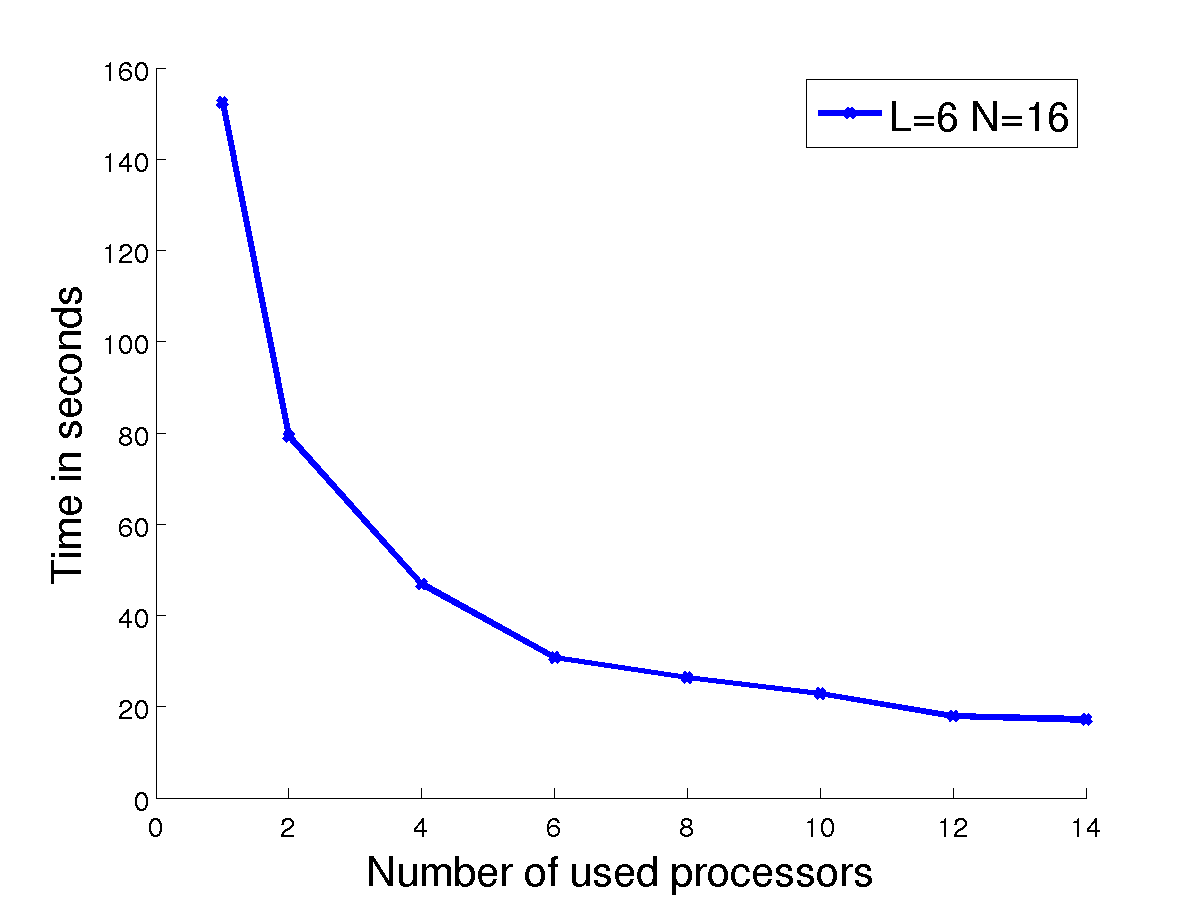
\includegraphics[height=40mm]{figures/strongscalingfulltiming.png}
        \label{fig:sub:strongscalingfulltiming}
    }
    \subfigure[Efficiency]{
        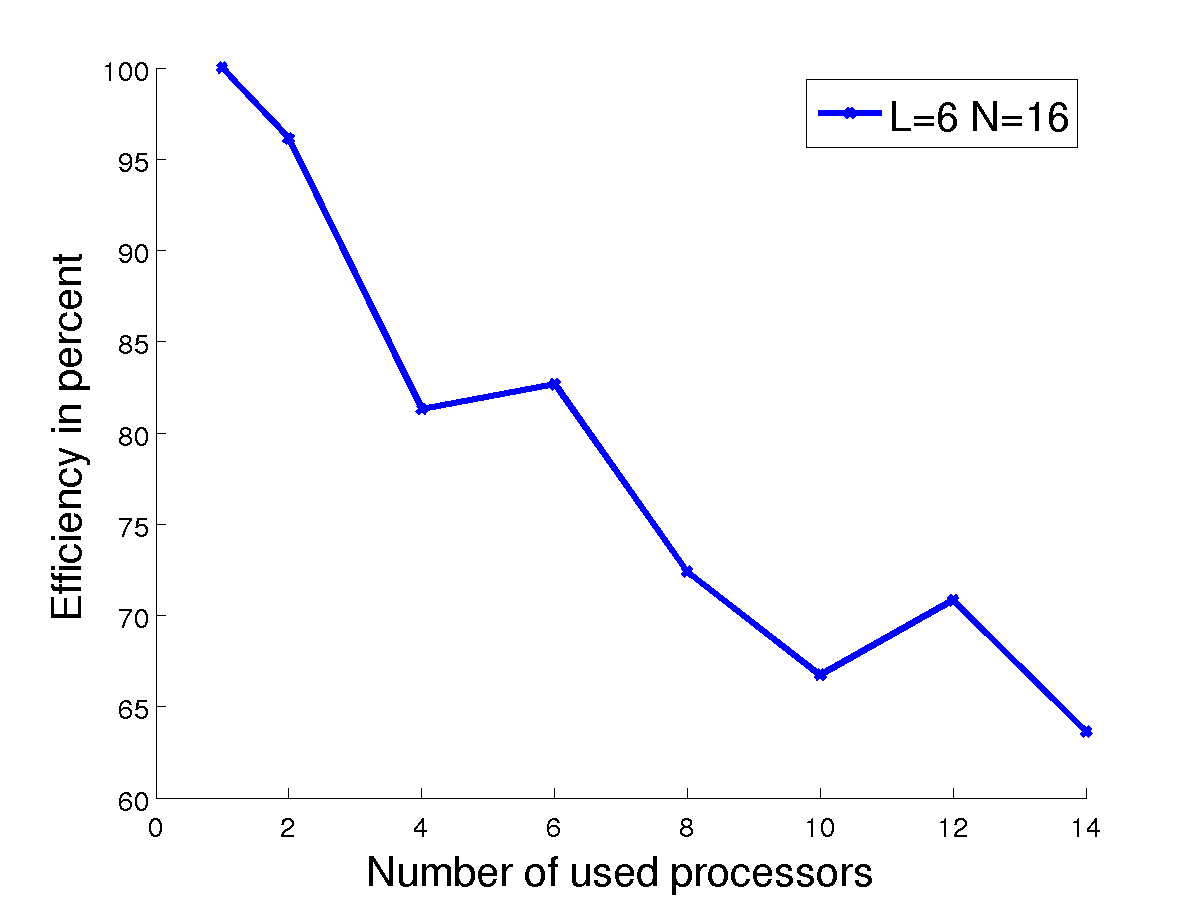
\includegraphics[height=40mm]{figures/strongscalingfullefficiency.png}
        \label{fig:sub:strongscalingfullefficiency}
    }
    \caption{Strong scaling of the RTE solver with the full tensor method. On the left the timing results are shown, on the right the according efficiency numbers are plotted.}
    \label{fig:strongscalingfull}
\end{figure}

\subsubsection{todocontent}
The todocontent environment is a customizable outline environment to help making the outline of a text.
\begin{todocontent}
    \1 This chapter should contain information about cows
    \1 And not to forget milk!
\end{todocontent}
